Aujourd'hui, nous allons voir les bases du C\# et de la POO. L'objectif est de se familiariser avec la syntaxe du C\# et de comprendre le fonctionnement de la programmation orientée objet (POO). Pour cela, vous allez devoir dans un premier temps implémenter des fonctions classiques puis créer des classes et manipuler celles-ci.

\begin{center}
  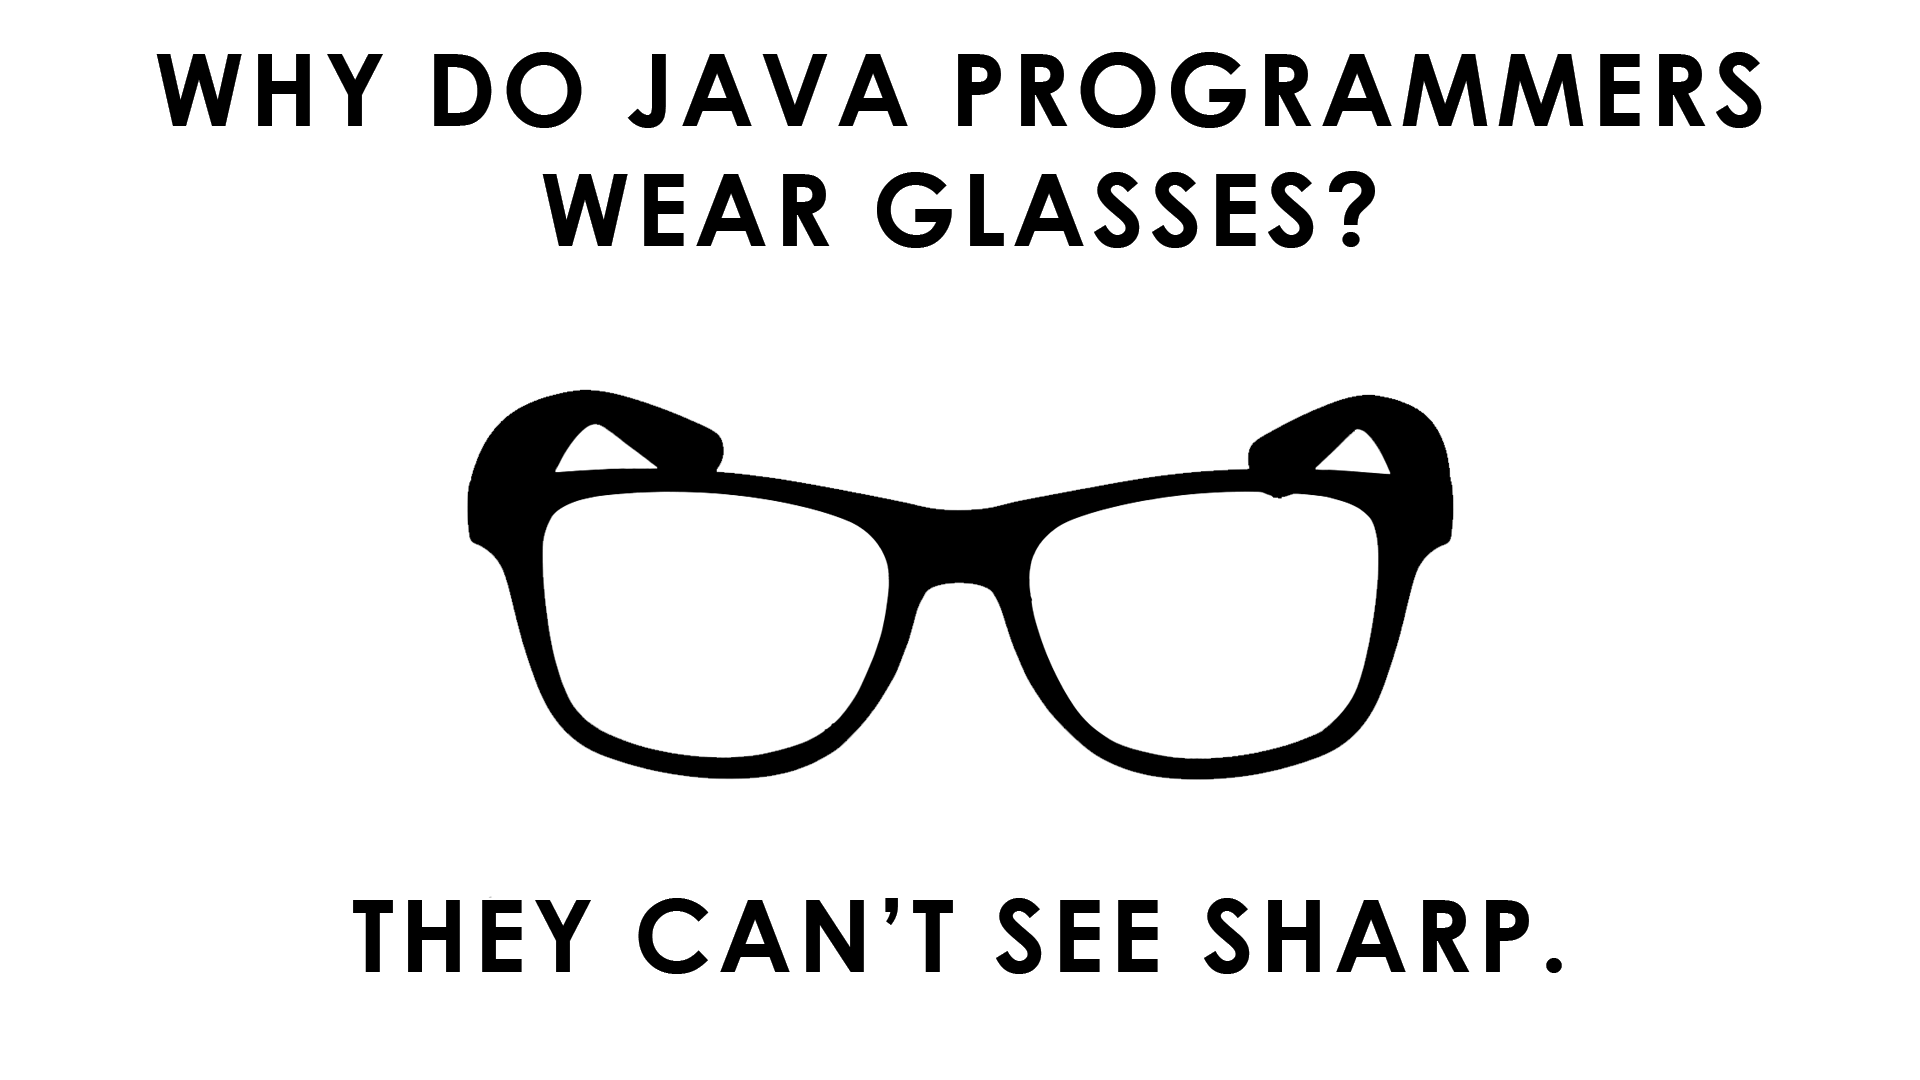
\includegraphics[width=\textwidth]{img/intro.png}
\end{center}